\documentclass{school-22.101-notes}
\date{October 26, 2011}

\begin{document}
\maketitle


\topic{Phase Shifts}
We want to show that phase shift converges; that is, if we fix $k$, and an increasing $l$ should lead to a decreasing $\delta_l$. 

A phase shift $\delta_l$ is defined in the above section in Eq.~\ref{delta_l}. We can determine $\delta_l$ analytically \footnote{try using the trigonometry $\sin(a+b) = \sin(a) \cos (b) + \cos(a) \sin(b)$?}. Keep in mind that $\delta_l$ is the phase shift for each of the partial wave that can scatter. It is a result of a partial wave interacting with the potential.  
\begin{figure}[ht]
    \centering
    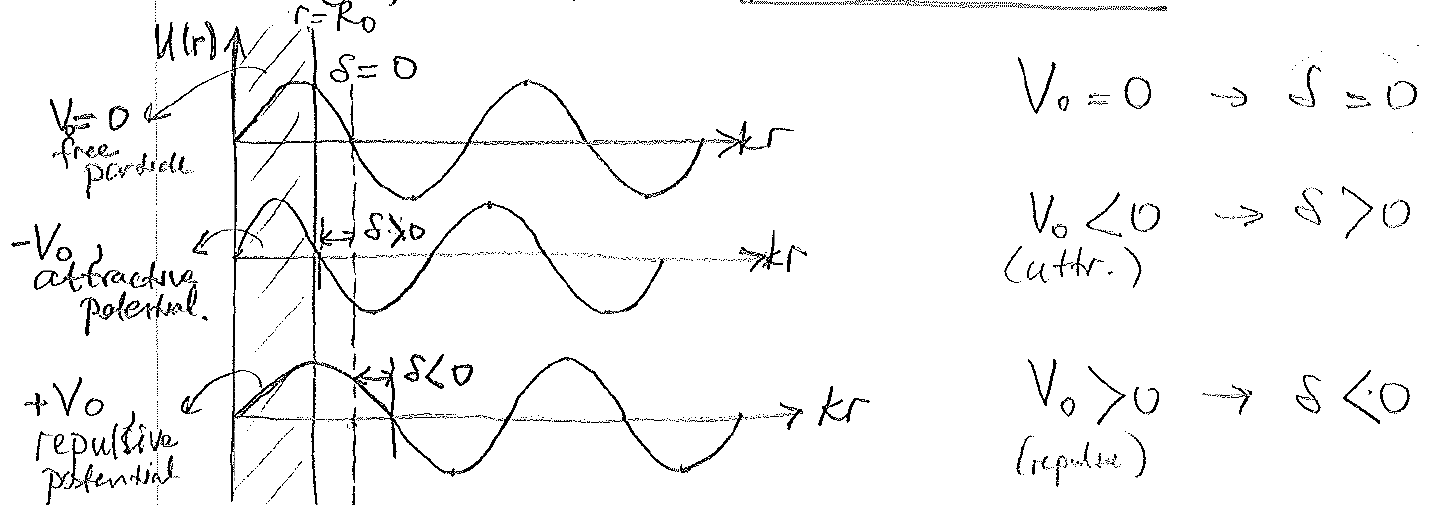
\includegraphics[width=6in]{images/scattering/scattering-potential-phase-shift.png}
    \caption{Phase Shift, Scattering Length }
\end{figure}

\topic{Low Energy S-Wave Approximation ($l=0$)}
\begin{figure}[ht]
    \centering
    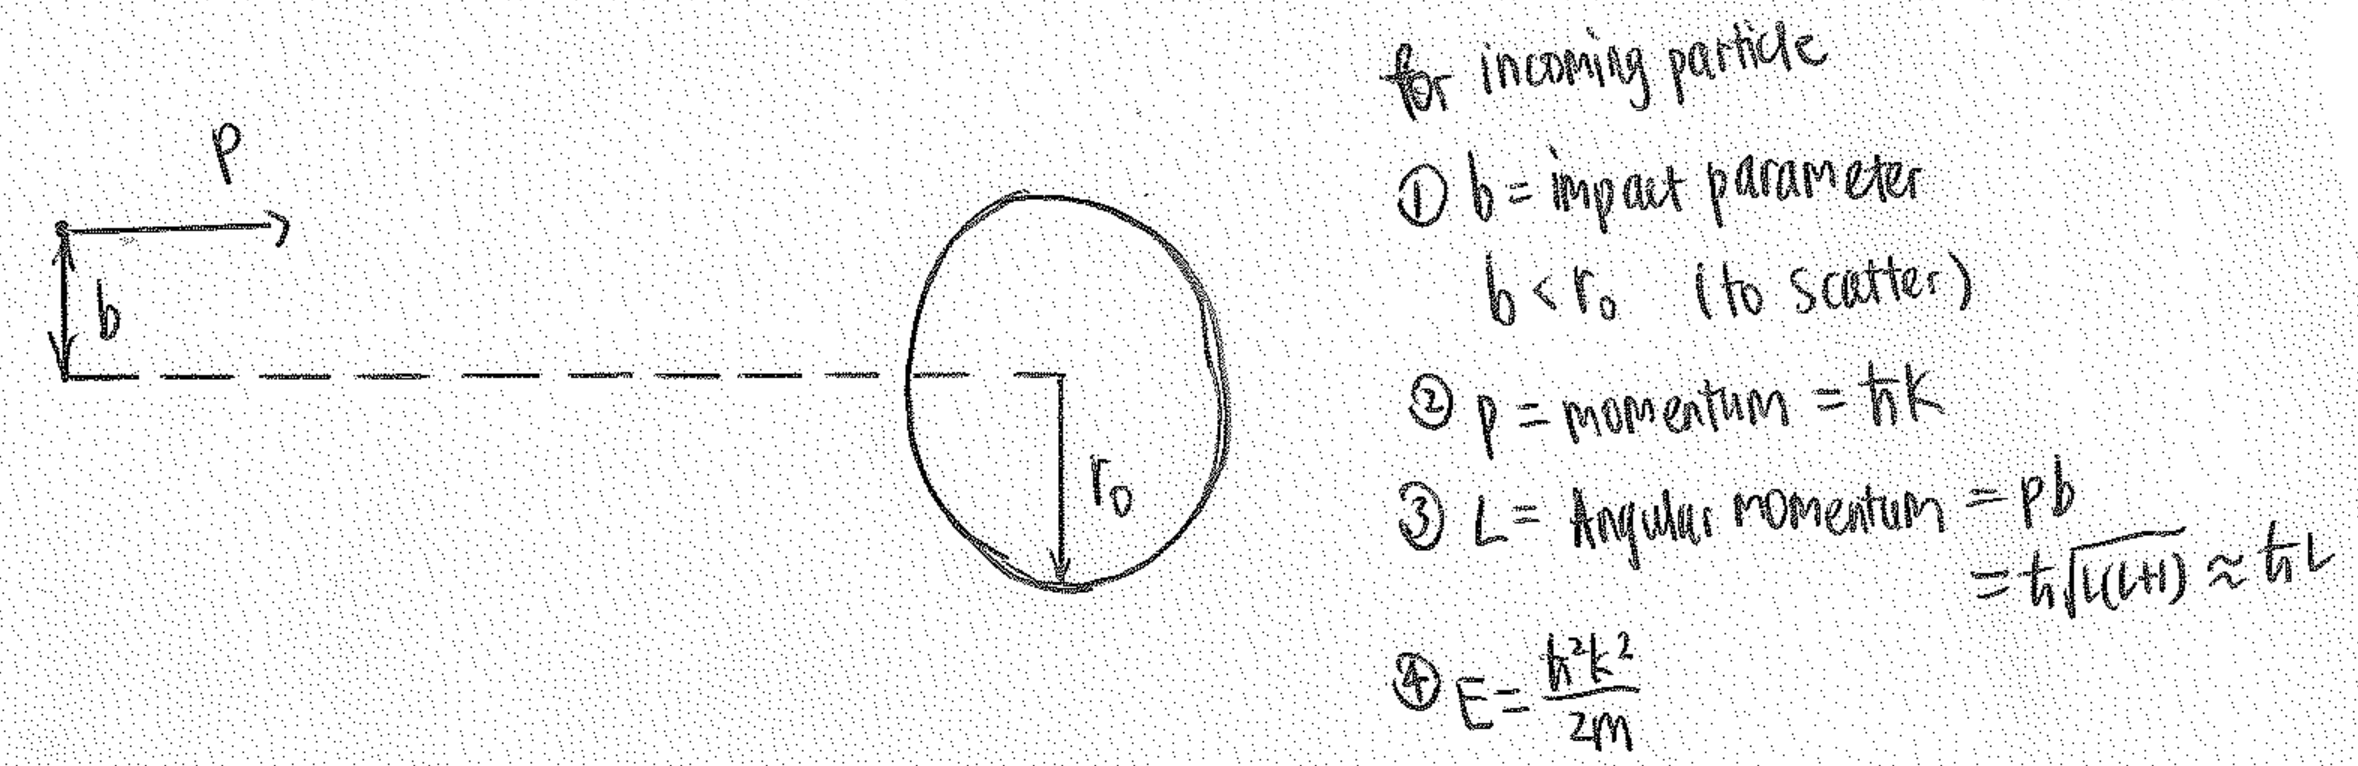
\includegraphics[width=4in]{images/scattering/np-scattering-diagram.png}
    \caption{n-p Scattering Diagram, S-Wave Approximation}
\end{figure}
\begin{enumerate}
\item A particle coming with a small incoming energy E means $k r_0 \ll 1$. This is because $E = \frac{\hbar^2 k^2}{2m} \Rightarrow k = \frac{\sqrt{2mE}}{\hbar}$, so when $E$ is small, $k$ is small. Similarly $r_0$ is reasonably small as well, hence $k r_0 \ll 1$. 

\item $ p = \hbar k$. 

\item $l=0$ because $l<kr_0 \ll 1$:
\begin{align}
L &= pb = \hbar \sqrt{l (l+1)} \approx \hbar l \Rightarrow \hbar l = pb = \hbar k b \\
\Rightarrow b &= \frac{l}{k} < r_0 \Rightarrow l < kr_0 \\
l &< k r_0 \ll 1 \Rightarrow l = 0
\end{align}

\item This is called a S-Wave Approximation. $\sigma (\theta), \sigma$ are simplified when $l=0$:
\begin{align}
\sigma (\theta) &= \frac{1}{k^2} \sin^2 \delta_0 & \sigma &= \boxed{ \frac{4 \pi}{k^2} \sin^2 \delta_0 } \label{sigma}
\end{align}

\item Observation: $\sigma$ is spherically symmetric, isotropic, because we assumed no $\theta$ dependency in S-Wave approximation. Example: when $E \approx 1 \fsp \eV \sim 10^4 \fsp \eV, \sigma = 20 \fsp b$. 

\item \textbf{Scattering Length $a$}: In the limit of low E, we define scattering length as\footnote{$a$ may be positive or negative. Here we use Krane's notation.}:
\begin{align}
\left. \begin{array}{c}
- \lim_{k\to 0} f(\theta) = a  \\
f(\theta) = \frac{1}{k} \Sum (2l+1) e^{i \delta_0} \sin \delta_0  P_l (\cos \theta) = \frac{1}{k} e^{i\theta_0} \sin \theta_0  \approx \frac{\delta_0}{k} 
\end{array} 
\right\} \Rightarrow \delta_0 = -ak
\end{align}
\begin{align}
\sigma &= 4 \pi \frac{1}{k^2} \sin^2 \delta_0 \approx 4 \pi \frac{\delta_0^2}{k^2} =  4 \pi \frac{(-ak)^2}{k^2} = 4 \pi a^2 \\
u(r) &= \frac{A_0}{k} \sin(kr + \delta_0) = \frac{a_0}{k} \sin (k(r-a)) \xrightarrow{\mathrm{small \fsp k}} \frac{a_0}{k} (k(r-a))
\end{align} 
The above expression suggests that $a$ behaves like an intercept.

\begin{figure}
    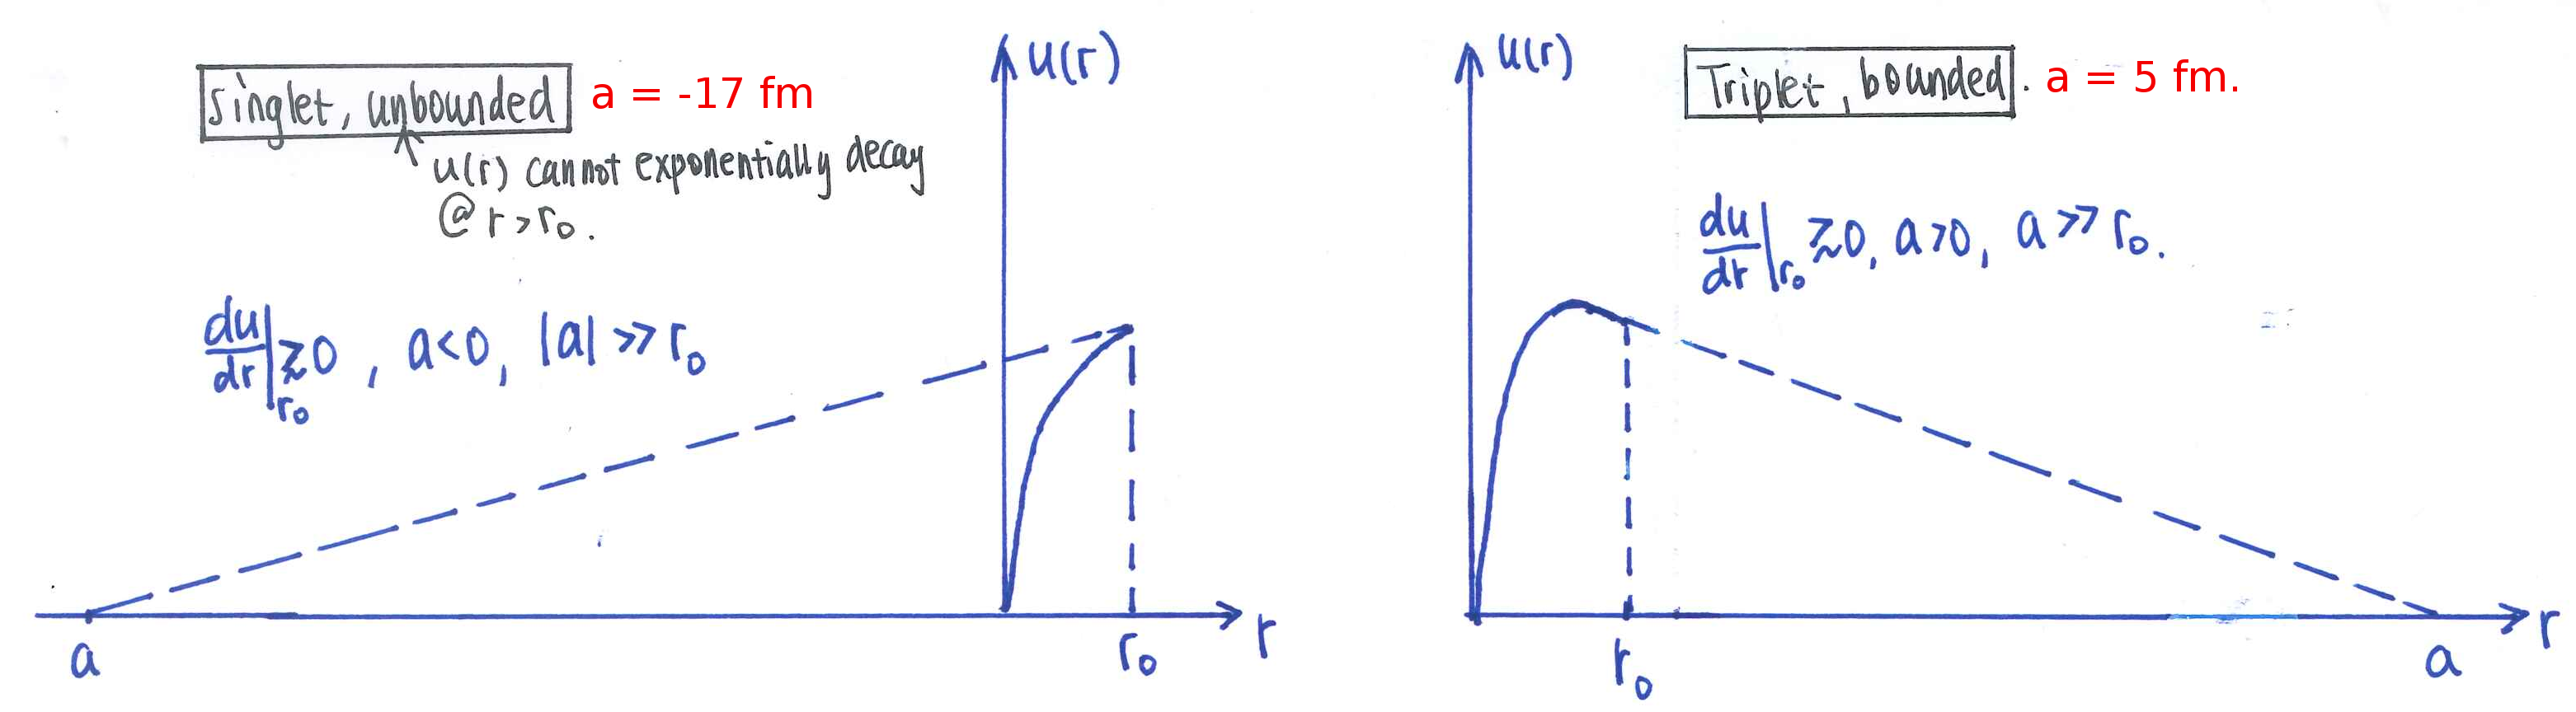
\includegraphics[width=7in]{images/scattering/s-wave-singlet-triplet.png}
    \caption{Singlet vs. Triplet Configuration for Low Energy ($E<10 \fsp \mathrm{keV}$)\label{scattering-s-wave}}
\end{figure}
Implications of Figure~\ref{scattering-s-wave}:
\begin{itemize}
\item Sign of $a$:  positive $a$ refers to triplet/bound state, negative $a$ refers to singlet/unbounded state. 
\item $a \gg r_0$. 
\item $a$ is `scattering amplitude' because 
\eqn{ \psi_{\mathrm{sc}} = f_0 \frac{e^{ikr}}{r} = \frac{\delta_0}{k} \frac{e^{ikr}}{r} = -a \frac{e^{ikr}}{r}  }
\end{itemize}
\end{enumerate}

\uline{Alternative approach to low energy s-wave} presented by Prof. Li on 10/24/12: as $k\to 0$, only $l=0$ term is important. The SEQ is, 
\eqn{ (\laplacian + k^2) \psi(x) = \frac{2 \mu V(x) \psi(x)}{\hbar^2} } 
Then we arrive at the Lippmann-Schwinger equation, 
\eqn{ \psi(x) = e^{ikx} - \int \dx'^3 \frac{e^{ik|x-x'|}}{4\pi |x-x'|} \frac{2 \mu V(|x'|) \psi(x') }{\hbar^2} }
Notice we arrive at an equation of $\psi(x)$ that depends on $\psi(x)$. We iterate, that is, we plug $\psi(x') = e^{ikx'}$ to solve for $\psi(x)$ and plug back in again. If we only iterate once and ignore $O(V^2)$, then we arrive at the \textbf{First Boron Approximation}, 
\eqn{ \psi(x) = e^{ikx} - \int \dx'^3 \frac{e^{ik|x-x'|}}{4\pi |x-x'|} \frac{2 \mu V(|x'|) e^{ikx'} }{\hbar^2} }
In the limit of low energy scattering ($k \to 0$), the wave is of central/spherical, that is, $f(\theta)$ is a constant. More specifically, we can see that in low energy s-wave approximation, 
\eqn{ \lim_{k\to 0} f(\theta) = \lim_{k\to 0} \frac{1}{k} e^{i\delta_0} \sin \delta_o = \frac{\delta_0}{k} }
We define a scattering length $a$ that satisfies 
\eqn{ a = \lim_{k\to 0} \frac{-\delta_0}{k} }
Thus $f(\theta) = -a$. Then the wavefunction is, 
\eqn{ \psi (x) = e^{ikx} - a \frac{e^{ikr}}{r} }
and the total scattering cross section is,
\eqn{ \sigma = \lim_{k\to 0} 4 \pi \frac{\delta_0^2}{k^2} = 4 \pi a^2}


Next we consider many scatters. We assume that there is no overlap between different scatters, and the scatterings are well separated, so we can use superposition. The wavefunction comes out to be,
\eqn{ \psi(x) = e^{ikx} - \left[ \Sum_m a_m e^{i (k-k_{\mathrm{out}}) \cdot x_m} \right] \frac{ e^{ikr}}{r} }
Comments: 
\begin{itemize}
\item Many scatters are not isotropic anymore because of the interference. 
\item The sign of $a$ does not matter for $\sigma$ in the case of single scatter. But with multiple scatters, the signs of each $a$ would matter. 
\item We define a $\displaystyle q = k_{\mathrm{out}} - k = k(\hat{x} - \hat{e}_z), S(q) = \Sum_m a_m e^{-i q \cdot x_m}$, so 
  \eqn{ \psi_{\mathrm{scatter}} (x) = - S(q) \frac{e^{ik|x|}}{|x|} }
  This is the basis of particle scattering. Setting up detectors at different location would tell us information about the structure of the nuclides. The readings on the detector is the intensity $I(q) \propto |S(q)|^2$. 
\end{itemize}


We consider the well problem again and solve the SEQ. After derivation,  
\eqn{ R - a &= \tan (k_0 R) / k_0 & a &= R - \frac{\tan(k_0 R)}{k_0} }
We can plot $a$ as a function of $k_o R$ and observes: 
\begin{itemize}
\item $V_0 = 0, k_0 = 0, \Rightarrow a= 0 ,\sigma = 0$. 
\item As $V_0 \up, k_0 \up, a$ becomes negative during $k_0 R \in [0, \frac{\pi}{2}$. 
\item $k_0 R = \frac{\pi}{2}, a = -\infty, \sigma = \infty$, we hit resonances. A subtle point here is that the curve ($a$ vs. $k_0 R$ which is effectively cross section as a function of well depth) looks very similar to the resonance scattering cross section plot with respect to energy. While the two plots are not quite the same thing, they do have the same underlying principle in the sense that $E$ and $V$ show up in the SEQ as a single term $E-V$.  
\item $k_0 R \in [\frac{\pi}{2}, \pi]$, $a$ is positive. 
\item $k_0 R$ approaches $\pi$, $a = 0$, the particle is effectively invisible. 
\end{itemize}


Scattering experiments, we consider shotting a neutron at a neutron, shotting a proton at a neutron, shotting a proton at a proton: 
\begin{itemize}
\item $\displaystyle a^{\mathrm{singlet}}_{nn} = -16.6 \fm$. 
\item $\displaystyle a^{\mathrm{singlet}}_{pp} = -7.82 \fm$. If we remove the Coulomb effect, $\displaystyle \tilde{a}^{\mathrm{singlet}}_{pp} = -17.1 \fm \sim a^{\mathrm{singlet}}_{nn}$. This is called `charge' symmetry. 
\item $\displaystyle a^{\mathrm{singlet}}_{np} = -23.72 \fm$, which is called `nearly charge' independency. 
\item $\displaystyle a^{\mathrm{triplet}}_{np} = 5.423 \fm$. There is only 1 weakly bound state. 
\end{itemize}

\end{document}
